\chapter{The Modules}

\section{Satellite super module}
The satellite super-module (internally represented by the class NSatellite) provides an interface to all other satellite modules, which are required by various other simulation and analysis modules.
\subsection{Orbit engine}
The orbit engine provides information about the current orbit position of the satellite, e.g. altitude, inclination, position in TBD coordinates.

\subsection{Pointing engine}
\begin{figure}[tb]
\begin{center}
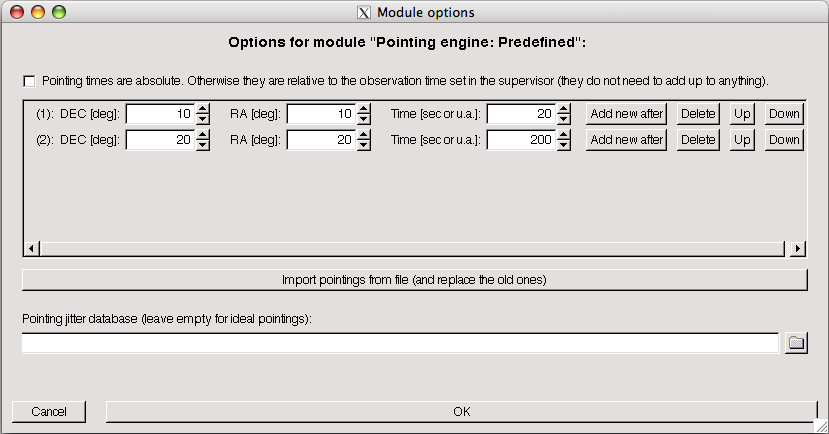
\includegraphics[width=10cm]{images/pointingGUI.png}  
\caption{Pointing module options GUI.}
\label{pointinggui} 
\end{center}
\end{figure}
The pointing engine provides the pointing of the focal plane module in declination and right ascension. Figure \ref{pointinggui} shows the options interface GUI for the pointing module. As illustrated the pointing module allows the user to define multiple pointings. Each pointing requires a coordinate set, a space craft roll, and an exposure time. Checking the box in the upper left turns the exposure times into absolute seconds, where as leaving it unchecked, the times become relative to the integration time given by the supervisor.

\subsection{Orientation and alignment engine}
\begin{figure}[tb]
\begin{center}
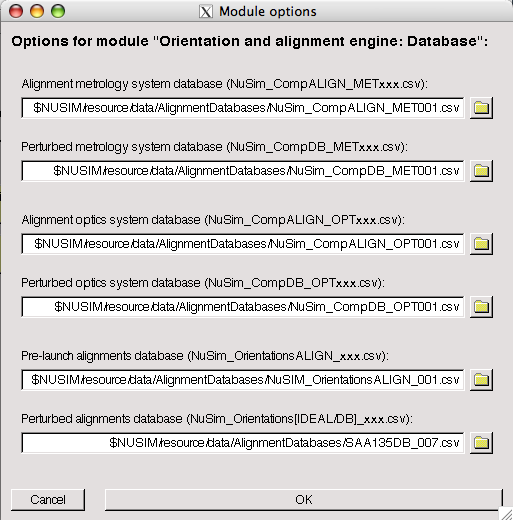
\includegraphics[width=10cm]{images/DBgui.png}  
\caption{Database and alignments options GUI.}
\label{dbgui} 
\end{center}
\end{figure}

The database and alignments module controls input databases and Figure \ref{dbgui} shows the interface options GUI. Each database entry comes in two forms: the ideal alignment of the system as defined "pre-flight", and the "in-flight" alignments which will be subject to thermal perturbations. The databases are divided into 3 groups: the optics, the metrology and star tracker, and finally the rest of the spacecraft alignments. The optics, metrology and star tracker are kept separate so that they can be changed frequently without having to redo the other databases.

\subsection{Time engine}
At the moment the time engine provides the absolute time of the satellite. Modules such as the detector module, the metrology and star tracker module derive their own time from this absolute satellite time and transfer it to the event, star tracker and metrology data sets.   

\subsection{Geometry and detector properties} 

\section{Event pipeline}

\subsection{Source engine}
\begin{figure}[tb]
\begin{center}
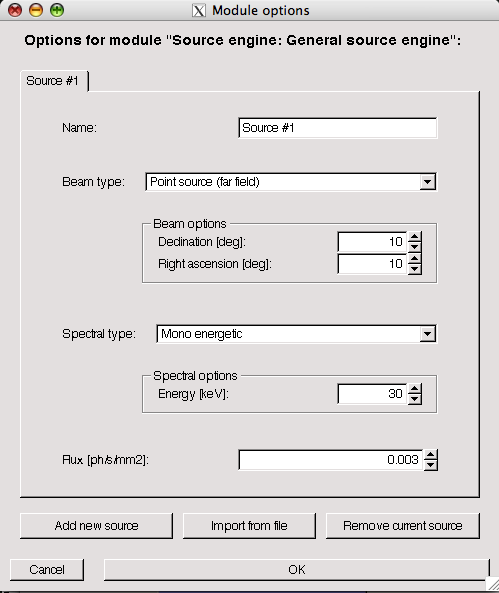
\includegraphics[scale=0.5]{images/sourceGUI.png}  
\caption{Source module options GUI.}
\label{sourcegui} 
\end{center}
\end{figure}
The source module generates the initial spatial and spectral photon distribution for the simulator. Figure \ref{sourcegui} shows the options interface GUI for the source module. Multiple sources can be generated and each source needs to have specified a beam type, spectral type and a flux. It is important to note the the flux here is in (ph/cm$^2$/s). In addition, the flux is always the integrated flux within the given energy bounds set with the spectral options.  

You need to set four parameters for a source: its name, its beam type, its spectral type, and its flux.

The beam type defines the geometry and the position of the source. The position is absolute and in degrees. Make sure that the source and telescope pointing matches. The following beam types are available:
 \begin{itemize}
 \item \textbf{Point source (far field)}: This is a point source at infinity. It requires RA and DEC coordinates in degree.
 \item \textbf{Disk source (far field)}: This creates a disc at infinity defined by its radius. It requires RA and DEC coordinates in degree as well as the radius of the disk in degree.
 \item \textbf{Point source (near field)}: This is used for mimicking a calibration source at a finite distance above the detector. It requires the position of the source (x, y, z in mm).
 \item \textbf{Pencil beam (near field)}: This beam is used to verify CZT detector calibrations. The pencil beam requires a start position as well as a direction (x, y, z in mm), as well as the radius of the beam.  
 \item \textbf{Read from fits file}: This creates a photon field based on a fits intensity image.
 \end{itemize}
 
The spectral options are:
\begin{itemize} 
\item \textbf{Mono-energetic}: Requires only the line energy in keV.
\item \textbf{Linear}: Requires the upper and lower boarder of the energy range in keV.
\item \textbf{Power-law}: Requires the upper and lower boarder of the energy range in keV as well as the photon index.
\item \textbf{Broken power-law}: Requires the upper and lower boarder of the energy range in keV, the break energy in keV, as well as the lower and upper photon index.
\item \textbf{Black body}: Requires the upper and lower boarder of the energy range in keV as well as the temperature in keV.
\item \textbf{File with differential flux}: Read differential spectrum from an ASCII file. The spectrum does not require any special normalization besides being 1/keV, since the total flux is as always given by the flux keyword. An example file of the format can be found at:\\
\textbf{\${NUSIM}/resource/data/SourceGenerator.examplespectrum.dat}
\end{itemize}

The final required parameter is the flux in $ph/cm^2/s$. This format instead of e.g. $ph/cm^2/s/keV/sr$ had to be chosen to allow to combine each spectrum with each beam. Therefore don't forget to integrate over keV, if you use non-mono-energetic spectra which are given in $keV^{-1}$.


For the sources at infinite distance the photons are started randomly from a disk on a sphere surrounding the opening of the optics modules (the module is chosen randomly) to enable the correct simulation of the effective area as a function of incidence angle. The start time is randomly determined (Poisson distribution) according to the source flux. When the start position, start direction and photon energy are determined, the photon is handed over to the optics module for further simulation.


\paragraph{Known issuses} 

\begin{itemize}
\item If you have too many sources then no tab is displayed in the GUI. This is a ROOT issue within the TGTab class. If you have too many sources it can on some systems take a long time to dispaly the GUI. This is another ROOT issue within the TGTab class.
\item If you change the beam or spectral type, all parameters get reset
\item Stay away from having sources close to the zenith or nadir (RA, DEC is 0 or 180 degrees) 
\end{itemize}

\vskip 10 true mm

\begin{figure}[tb]
\begin{center}
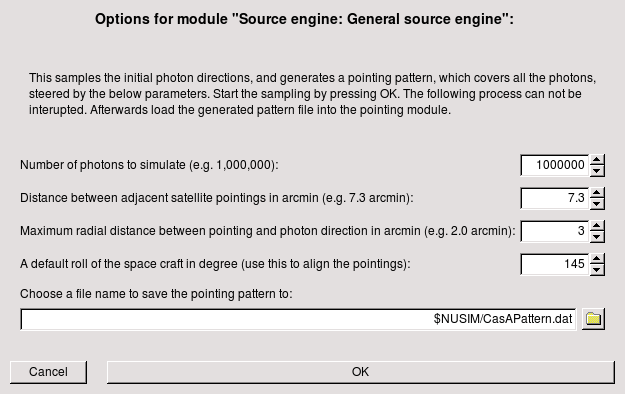
\includegraphics[scale=0.5]{images/pointingpatternGUI.png}  
\caption{GUI for generating pointing patterns.}
\label{pointingpatterngui} 
\end{center}
\end{figure}

A special feature of the source engine is that it can also generate a simple pointing pattern. To do so press the button "Pointing" in the source engine GUI and the GUI see in Fig \ref{pointingpatterngui} should appear. 

The pointing pattern is generated by first simulating a set of photons. The number of photons is given in the first entry box. It should be high enough to sample all sources, but not too high because then the simulation takes too long. 1,000,000 photons seems a reasonable compromise for most situations. For each photon the start direction in RA and DEC is stored. After the simulation, the source region is covered with a rectangular pattern of pointings. The distance between the pointings is given in the second entry field. Since the source field is not necessary rectangular many individual pointings may be not necessary. The last entry in GUI determines how close the pointing direction (i.e. the optical axis of the instrument) must be to a simulated photon in order to accept the pointing. A value of, e.g., 3 arcmin means that one photon must have been simulated within a radius of 3 arcmin of the pointing direction of the instrument. Don't make the value too small, otherwise it's unlikely you have simulated a photon within the disk, and do not make it larger than the half the field-of-view of the instrument.
The next input box gives the roll of the space craft, which allows to align the field-of-view (by trial and error at the moment).  
In the bottom entry box you give the name of the file to which the pointings are stored. You have to read this file in the pointing module in order to use it. 

In order to test and verify the coverage of your generated pointing pattern, as well as the evenness of your image, you can make a full simulation with a flat input distribution, e.g. a disk source, which is large enough to cover all pointings.



\subsection{Optics engine}
The optics engine is a full-fledged ray-trace to simulate the actual optics. It incorporates the exact geometry of the optics, and uses externally generated reflectivity files to calculate the reflection of the photons off the mirrors. Additionally it has a module to simulate deflection of the X-ray photons due to mirror imperfections, which will generate the mirror point spread function. The ray-trace also keeps track of single reflections, called "ghost rays", where the photon only reflects off one mirror while passing through.

The module has three options:
\begin{itemize}
\item \textbf{Scattering}: This options turns on the scattering of the photons due to figure errors in the mirrors. Scattering must be on for a science simulation. It is important to note that this is scattering in the reflection sense only, and not of any particle effects.
\item \textbf{Perfect Optics}: This option focuses all rays to one spot. This option should not be used with science simulations and is primarily for debugging.
\item \textbf{Ghost rays}: This option enables the ghost rays. As a default it should be on when running a science simulation. 
\end{itemize}

The input of this module is a photon location, direction and energy handed to it by the source module, and the output is location, direction and energy after the photon has exited the optics.


\subsection{Aperture engine}
The aperture engine places an aperture in the photon path and rejects any photon hitting the aperture. The aperture stop is located 833.187 mm above the detector, and has an opening diameter of 58 mm.

\subsection{Background engine}
\begin{figure}[tb]
\begin{center}
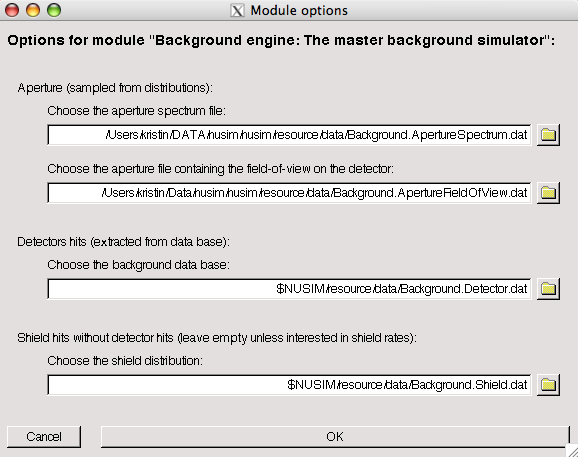
\includegraphics[width=8cm]{images/backgroundgui.png}  
\caption{Background interface options GUI for the "master background simulator".}
\label{bkggui} 
\end{center}
\end{figure}
The background engine draws the background from an external GEANT simulation, combining it with the expected background flux from the sky. This module has four options:
\begin{itemize}
\item \textbf{No Module}. It is possible to run NuSIM without having a background engine.
\item \textbf{Master Background Simulator}. As the name implies this is the actual background option to use when running science simulations. Figure \ref{bkggui} shows the interface options GUI and the files can be found in \textbf{\${NUSIM}/resource/data/}.
\item \textbf{Event Loader: Universal loader}. Allows the user to load a previously saved event list.
\end{itemize}
\subsection{Detector interactions engine}

\subsection{Detector effects engine}

\subsection{Trigger engine}
The trigger module represents the trigger and downlink decision hardware aboard the NuSTAR satellite. It shall decide if an energy deposit in the shield represents a veto or the pattern on the detector is valid for a downlink.

\subsection{Detector data calibrator}

\subsection{Event selector}

\subsection{Science analyzer}

\section{Metrology and Star tracker pipeline}
\subsection{Metrology engine and calibrator}
The purpose of the metrology engine is to generate data at a rate equivalent to the onboard metrology system. The engine takes the known perturbed aspect of the instrument system and finds the intersection of the metrology laser with the metrology detector. It will then apply noise to the data set simulating the centroiding error of the metrology detector. This is done by applying a Gaussian error to each of the measurement axis. The 1-sigma error is reported in the database file:\\ \textbf{resource/AlignmentDatabases/NuSim\_CompDB\_MET001.csv} . 

The engine passes the coordinates on to the Observatory Reconstructor for use in deriving the aspect reconstruction.

\subsection{Star tracker engine and calibrator}
Based on the input pointing defined by the pointing engine, the task of the Star Tracker Engine is to generate a quaternion, which defines the rotation between the Camera Head Unit, CHU, to the J2000.0 heliocentric inertial equatorial reference frame, also called VSN (Vernal, Summer, North). The origin is the intersection of the CCD plane with the optical axis of the camera. The CHU z-axis points along the boresight, and x/y axis span the CCD plane.
The output of the Star Tracker is a Quaternion that defines the attitude of the CHU w.r.t. the VSN, such that
\begin{equation} 
x_{CHU}=(Q_{CHU->VSN}) * x_{VSN}. 
\end{equation}
Thus if the a unit vector in the star tracker frame is transformed into the VSN frame by 
\begin{equation}
x_{VSN}=(Q_{CHU->VSN} )^T* x_{CHU}, 
\end{equation}
then RA=atan$(y_{VSN}/x_{VSN})$, DEC=acos$(z_{VSN})$. In the module $(Q_{CHU->VSN})^T$ is produced at a rate equivalent to the onboard Star Tracker. The module will add a Gaussian noise to the transformation to mimic solution error of the Star Camera. The 1-sigma error is reported in the database file:\\ \textbf{resource/AlignmentDatabases/NuSim\_CompDB\_MET001.csv} .

 The transformation is passed on to the Observatory Reconstructor, which interpolates the transformation for a specific time and derives the aspect reconstruction.

\subsection{Observatory reconstructor}
The observatory reconstructor is the set of algorithms that solves the attitude and aspect problems of the NuSTAR observatory, given the metrology and star tracker data. The observatory reconstructor does not have access to the satellite module, which would contain the actual attitude and aspect of the observatory. It is responsible for re-calculating that attitude and aspect, given only a certain number of inputs, which are simulated satellite data.
The inputs to the observatory reconstructor are:
\begin{itemize}
\item The calibrated positions, in local coordinates, at which the metrology lasers impinge on their detectors. These are interpolated in time.
\item The calibrated star tracker data, which is a transformation (quaternion) from local star tracker coordinates to inertial (J2000.0) coordinates. These are interpolated in time. 
\item The on-ground alignment data defining the ideal locations of all the instrument components. Specifically, the pointing of the optical axis in optics bench coordinates, the location and pointing direction of the metrology laser in optics bench coordinates, the location and rotation to the metrology detector from focal plane bench coordinates and to the star tracker from optics bench coordinates.
\end{itemize}
The output from the observatory reconstructor is a transformation from focal plane module coordinates to celestial coordinate $R_{fbin}$.
For extensive details on this reconstruction, and the algorithm solution, see the memo “NuSTAR Pointing Reconstruction.”


\subsection{Observatory merger}
